\section{全局存在}
\label{sec:odeex-global}

状态空间是$\mathbb{R}^{n}$时，最大解只有一种走不到时间区间尽头的方式：范数趋于无穷。于是只要能预先证明解在任何有限时间段上有界，爆炸就被排除了，解会一直延续到右端给定的整个时间区间。这样的解称为\term{全局解}（global solution）。

\paragraph{爆炸快慢由增长速度决定}
先看标量自治方程，算出爆炸发生的时刻。设$f$在$[x_0,\infty)$上连续且为正，局部Lipschitz，解单调上升。由$\mathrm{d}t=\mathrm{d}x/f(x)$，走到无穷所需的时间是
\begin{equation}
 T=\int_{x_0}^{\infty}\frac{\mathrm{d}x}{f(x)}.
 \label{eq:odeex-blowup-time}
\end{equation}
这个积分有限时，解在$T$时刻爆炸；无穷时，解不爆炸。状态越大，箭头越快，走过单位状态所用的时间$1/f(x)$越短，这些时间加起来可能有限。

取$f(x)=x^p$，$x_0=1$。$p>1$时
\[
 T=\int_1^\infty x^{-p}\,\mathrm{d}x=\frac{1}{p-1},
\]
$p=2$时$T=1$，与前面的结果一致。$p=1$时积分发散，解是$\mathrm{e}^t$，增长虽快，但在有限时间内走不到无穷。线性增长正是这个分界线。图~\ref{fig:odeex-blowup-integral}(a)比较了$1/x^2$和$1/x$的尾部面积，图(b)比较了相应的解。

\begin{BookInlineFigure}
  \centering
  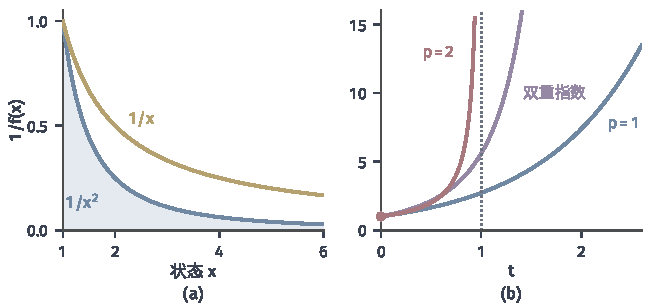
\includegraphics[width=112mm]{figures/06-differential-equations/01-ordinary-differential-equations/matplotlib/odeex-blowup-integral/figure.pdf}
  \caption{增长速度与有限时间爆炸。(a)走过单位状态的用时$1/f(x)$：蓝线$1/x^2$的尾部面积（浅蓝）有限，等于$1$；黄线$1/x$的尾部面积无穷。(b)初值都为$x(0)=1$的解：红线$\dot x=x^2$在$t=1$爆炸，蓝线$\dot x=x$是$\mathrm{e}^t$，紫线$\dot x=(1+x)\ln(1+x)$是$2^{\mathrm{e}^t}-1$，增长比线性快但不爆炸。}
  \label{fig:odeex-blowup-integral}
\end{BookInlineFigure}

\paragraph{至多线性增长}
线性增长是分界线，这一观察对向量方程仍然有用，只要把$\lVert\bm{f}\rVert_2$用状态范数的一次函数控制住。系数可以随时间变化，甚至只要局部可积。

\begin{theorem}[线性增长下的全局存在]
\label{thm:odeex-global}
设$J\subseteq\mathbb{R}$是开区间，$\bm{f}:J\times\mathbb{R}^{n}\to\mathbb{R}^{n}$连续，在状态方向局部Lipschitz连续且对时间局部一致。若存在$J$上局部可积的非负函数$\alpha,\beta$，使对所有$t\in J$，$\bm{x}\in\mathbb{R}^{n}$，
\begin{equation}
 \lVert\bm{f}(t,\bm{x})\rVert_2\leq\alpha(t)\lVert\bm{x}\rVert_2+\beta(t),
 \label{eq:odeex-linear-growth}
\end{equation}
则对每个$(t_0,\bm{x}_0)\in J\times\mathbb{R}^{n}$，最大解定义在整个$J$上，并且对$t\in J$，
\begin{equation}
 \lVert\bm{x}(t)\rVert_2\leq\Bigl(\lVert\bm{x}_0\rVert_2+\Bigl\lvert\int_{t_0}^{t}\beta\Bigr\rvert\Bigr)\exp\Bigl\lvert\int_{t_0}^{t}\alpha\Bigr\rvert.
 \label{eq:odeex-global-bound}
\end{equation}
\end{theorem}

满足式~\eqref{eq:odeex-linear-growth}的右端称为\term{至多线性增长}（at most linear growth）。证明分两步：先证明界~\eqref{eq:odeex-global-bound}，再用它排除爆炸。

\begin{proof}
设$\bm{x}$是最大解，定义在$(\omega_-,\omega_+)$上。先看$t\geq t_0$的一侧。取$T\in[t_0,\omega_+)$，记$u(t)=\lVert\bm{x}(t)\rVert_2$，它是$[t_0,T]$上的连续函数。由积分方程~\eqref{eq:odeex-integral}和式~\eqref{eq:odeex-linear-growth}，对$t\in[t_0,T]$，
\[
 u(t)\leq\lVert\bm{x}_0\rVert_2+\int_{t_0}^{t}\bigl(\alpha(s)u(s)+\beta(s)\bigr)\,\mathrm{d}s\leq B+\int_{t_0}^{t}\alpha(s)u(s)\,\mathrm{d}s,
\]
其中$B=\lVert\bm{x}_0\rVert_2+\int_{t_0}^{T}\beta$。

把右端记作$v(t)$，它在$[t_0,T]$上绝对连续，几乎处处有$\dot v=\alpha u\leq\alpha v$。令$A(t)=\int_{t_0}^t\alpha$，$A$也绝对连续。绝对连续函数的乘积仍绝对连续，于是几乎处处有
\[
 \frac{\mathrm{d}}{\mathrm{d}t}\bigl(v\,\mathrm{e}^{-A}\bigr)=(\dot v-\alpha v)\,\mathrm{e}^{-A}\leq0.
\]
绝对连续函数可由导数积分恢复，所以$v\,\mathrm{e}^{-A}$单调不增，由此
\[
 v(T)\leq v(t_0)\,\mathrm{e}^{A(T)}=B\,\mathrm{e}^{A(T)}.
\]
这里用到的绝对连续函数的性质，可参考\BookChapterRef{chap:integration}{卷四第6章“积分”}。由$u(T)\leq v(T)$，式~\eqref{eq:odeex-global-bound}在$t=T$处成立。

设$\omega_+<\sup J$。此时$[t_0,\omega_+]$是$J$的紧子集，$\alpha,\beta$在其上可积，所以式~\eqref{eq:odeex-global-bound}的右端对$T<\omega_+$有一个与$T$无关的上界。这与式~\eqref{eq:odeex-blowup-alternative}矛盾，于是$\omega_+=\sup J$。

$t\leq t_0$的一侧，令$\tilde{\bm{x}}(s)=\bm{x}(2t_0-s)$，它满足右端为$-\bm{f}(2t_0-s,\cdot)$的方程，增长条件的系数换成$\alpha(2t_0-s),\beta(2t_0-s)$，应用前面的结论即可。
\end{proof}

条件各有分工。式~\eqref{eq:odeex-linear-growth}是全局条件，要求对所有状态成立，正是它阻止了爆炸；Lipschitz条件只是局部的，它负责唯一性和最大解的存在，不参与防止爆炸。$\alpha,\beta$在紧时间段上可积，$\exp\int\alpha$才是有限数。

\paragraph{几个例子}
\begin{example}[线性系统]
\label{ex:odeex-linear-global}
设$\bm{A}(t)$和$\bm{g}(t)$在开区间$J$上连续，$\bm{f}(t,\bm{x})=\bm{A}(t)\bm{x}+\bm{g}(t)$。在紧时间段上$\lVert\bm{A}(t)\rVert_2$有界，
\[
 \lVert\bm{f}(t,\bm{x})-\bm{f}(t,\bm{y})\rVert_2\leq\lVert\bm{A}(t)\rVert_2\lVert\bm{x}-\bm{y}\rVert_2,
\]
满足局部Lipschitz条件。增长条件取$\alpha=\lVert\bm{A}(t)\rVert_2$，$\beta=\lVert\bm{g}(t)\rVert_2$，因此每个初值问题的解都定义在整个$J$上，这正是第~\ref{chap:linear-differential-systems}章的传播公式成立的范围。
\end{example}

\begin{example}[单摆]
\label{ex:odeex-pendulum-global}
单摆方程$\ddot x=-\sin x$写成状态$(x,v)$的系统，右端$\bm{f}(x,v)=(v,-\sin x)$是非线性的。由$\lvert\sin x\rvert\leq\lvert x\rvert$，
\[
 \lVert\bm{f}(x,v)\rVert_2=\sqrt{v^2+\sin^2x}\leq\lVert(x,v)\rVert_2.
\]
取$\alpha=1$，$\beta=0$，单摆的解对所有$t\in\mathbb{R}$存在，并满足
\[
 \lVert(x,v)(t)\rVert_2\leq\lVert(x_0,v_0)\rVert_2\,\mathrm{e}^{\lvert t\rvert}.
\]
\end{example}

\begin{example}[界与真解的比较]
\label{ex:odeex-barrier}
取$\dot x=\sqrt{1+x^2}$，$x(0)=0$，真解是$\sinh t$。由$\sqrt{1+x^2}\leq1+\lvert x\rvert$，可取$\alpha=\beta=1$，式~\eqref{eq:odeex-global-bound}给出，对$t\geq0$，
\[
 \lvert x(t)\rvert\leq t\,\mathrm{e}^{t}.
\]
在$t=1$处，界约为$2.718$，真解约为$1.175$。
\end{example}

图~\ref{fig:odeex-linear-growth-barrier}把这个界和真解画在一起，并与右端只多了平方项的$\dot x=1+x^2$对照。界比真解松得多，但它对每个有限的$t$都是有限数，这已足够排除爆炸；$\dot x=1+x^2$的解$\tan t$不满足线性增长条件，在$t=\pi/2$爆炸。

\begin{BookInlineFigure}
  \centering
  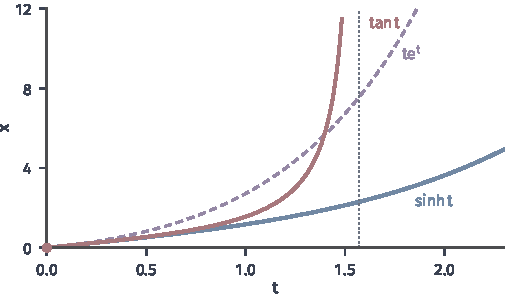
\includegraphics[width=88mm]{figures/06-differential-equations/01-ordinary-differential-equations/matplotlib/odeex-linear-growth-barrier/figure.pdf}
  \caption{线性增长下的上界。蓝线是$\dot x=\sqrt{1+x^2}$的解$\sinh t$，紫色虚线是由式~\eqref{eq:odeex-global-bound}得到的界$t\mathrm{e}^t$，红线是$\dot x=1+x^2$的解$\tan t$，在点线$t=\pi/2$处爆炸。初值都是$x(0)=0$。}
  \label{fig:odeex-linear-growth-barrier}
\end{BookInlineFigure}

\paragraph{条件的边界}
线性增长是充分条件，并不必要。前面图~\ref{fig:odeex-blowup-integral}(b)中的$\dot x=(1+x)\ln(1+x)$增长比线性快，令$y=\ln(1+x)$，方程化为$\dot y=y$，于是$x=2^{\mathrm{e}^t}-1$对所有$t$存在；由式~\eqref{eq:odeex-blowup-time}，这相当于$\int^{\infty}\mathrm{d}x/\bigl((1+x)\ln(1+x)\bigr)$发散。

符号也起作用。$\dot x=-x^3$的增长是三次的，但它把状态往零拉，解
\[
 x(t)=\frac{x_0}{\sqrt{1+2x_0^2t}}
\]
对所有$t\geq0$存在；向后走时，它在$t=-1/(2x_0^2)$爆炸。线性增长条件不看方向，所以它同时保证了两个时间方向的存在。

\paragraph{全局存在不是长期稳定}
定理~\ref{thm:odeex-global}只说解在每个有限时刻都有定义，不说解保持有界。$\dot x=x$的解$\mathrm{e}^t$全局存在，并趋于无穷；式~\eqref{eq:odeex-global-bound}的右端也随$t$增长。解的长期去向、是否靠近平衡点，要用另外的结构和条件来研究，可参考\BookChapterRef{chap:dynamical-systems-long-term}{卷九第1章“动力系统与轨迹的长期行为”}。

增长条件也不提供唯一性。式~\eqref{eq:odeex-sqrt}的右端满足$2\sqrt{\lvert x\rvert}\leq1+\lvert x\rvert$，是至多线性增长的，前面写出的解$x_c$对所有$t\geq0$都有定义，却有无穷多条。全局性与唯一性由不同的条件负责。
